\section{Steady-State Output Regulation}
\label{sec:res-steady}

The selected average output was maintained through the loaded sweep: up to
\SI{3}{\ampere} at \SI{5}{\volt}, \SI{9}{\volt}, and
\SI{15}{\volt}, and up to \SI{4}{\ampere} at \SI{20}{\volt}.
Average-voltage error was calculated as
\begin{equation}
e_V=\frac{V_\mathrm{BUS,avg}-V_\mathrm{set}}{V_\mathrm{set}}\,100\%,
\label{eq:steady-voltage-error}
\end{equation}
where \(V_\mathrm{BUS,avg}\) is the mean USB-C output voltage. The MCU
regulates the secondary bulk supply feeding the USB-C PD stage.

\begin{figure}[htbp]
\centering
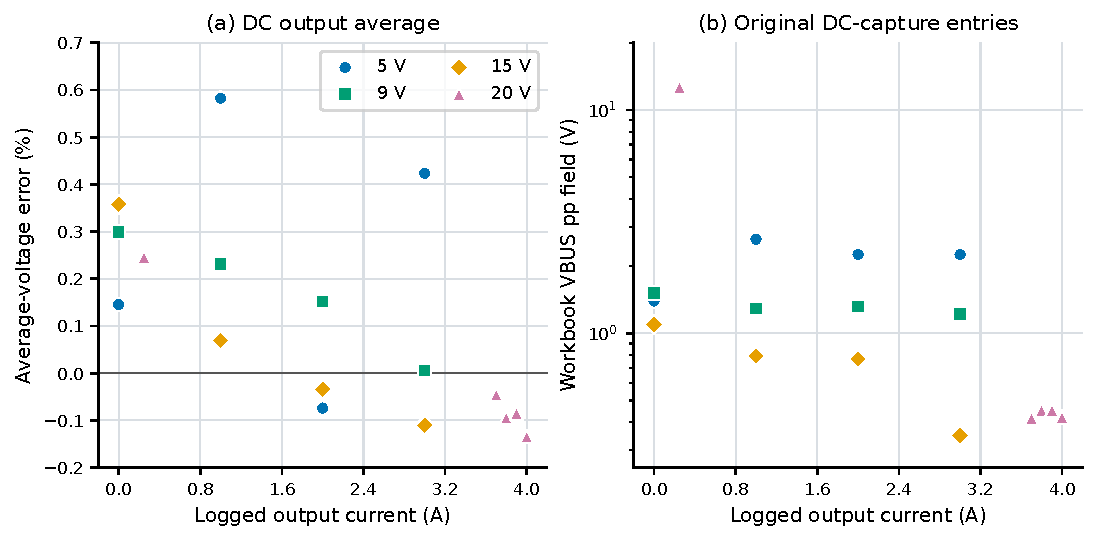
\includegraphics[width=\textwidth]{Pictures/Thesis/10_Results/Rebuilt/regulation_and_logged_ripple.pdf}
\caption{Measured output-voltage error and the workbook VBUS peak-to-peak readings. The right panel uses a logarithmic scale and includes the anomalous workbook values. AC-coupled statistics are plotted separately.}
\label{fig:rebuilt-regulation}
\end{figure}

The largest absolute loaded error was \SI{0.583}{\percent}, at
\SI{5}{\volt} and \SI{1}{\ampere}, with average VBUS of
\SI{5.02913}{\volt}. At maximum load for each lower-voltage setting, the
averages were \SI{5.02118}{\volt}, \SI{9.00057}{\volt}, and
\SI{14.9835}{\volt}. These averages show that the USB-C PD output remained close to its selected
voltage; ripple and transient limits require separate measurements.

\begin{table}[htbp]
\centering
\caption{Maximum-load and high-power measurements. Output power is calculated from average VBUS and load current. The pp column contains the original workbook readings.}
\label{tab:steady-state-results}
\small
\begin{tabular}{@{}rrrrrr@{}}
\toprule
Setting (V) & Load (A) & VBUS avg (V) & Error (\%) & Logged pp (V) & Output (W)\\
\midrule
5 & 3.0 & 5.02118 & +0.424 & 2.252 & 15.06\\
9 & 3.0 & 9.00057 & +0.006 & 1.220 & 27.00\\
15 & 3.0 & 14.98350 & $-0.110$ & 0.349 & 44.95\\
20 & 3.7 & 19.99090 & $-0.046$ & 0.416 & 73.97\\
20 & 3.8 & 19.98130 & $-0.094$ & 0.452 & 75.93\\
20 & 3.9 & 19.98320 & $-0.084$ & 0.453 & 77.93\\
20 & 4.0 & 19.97320 & $-0.134$ & 0.421 & 79.89\\
\bottomrule
\end{tabular}
\end{table}

At \SI{20}{\volt}, increasing load from \SI{3.7}{\ampere} to
\SI{4.0}{\ampere} reduced average VBUS by only \SI{17.7}{\milli\volt}
while calculated output rose from \SI{73.97}{\watt} to
\SI{79.89}{\watt}. The \SI{3.8}{\ampere} point exceeded \SI{75}{\watt} calculated output.

\begin{figure}[htbp]
\centering
\begin{subfigure}[t]{0.48\textwidth}
\centering
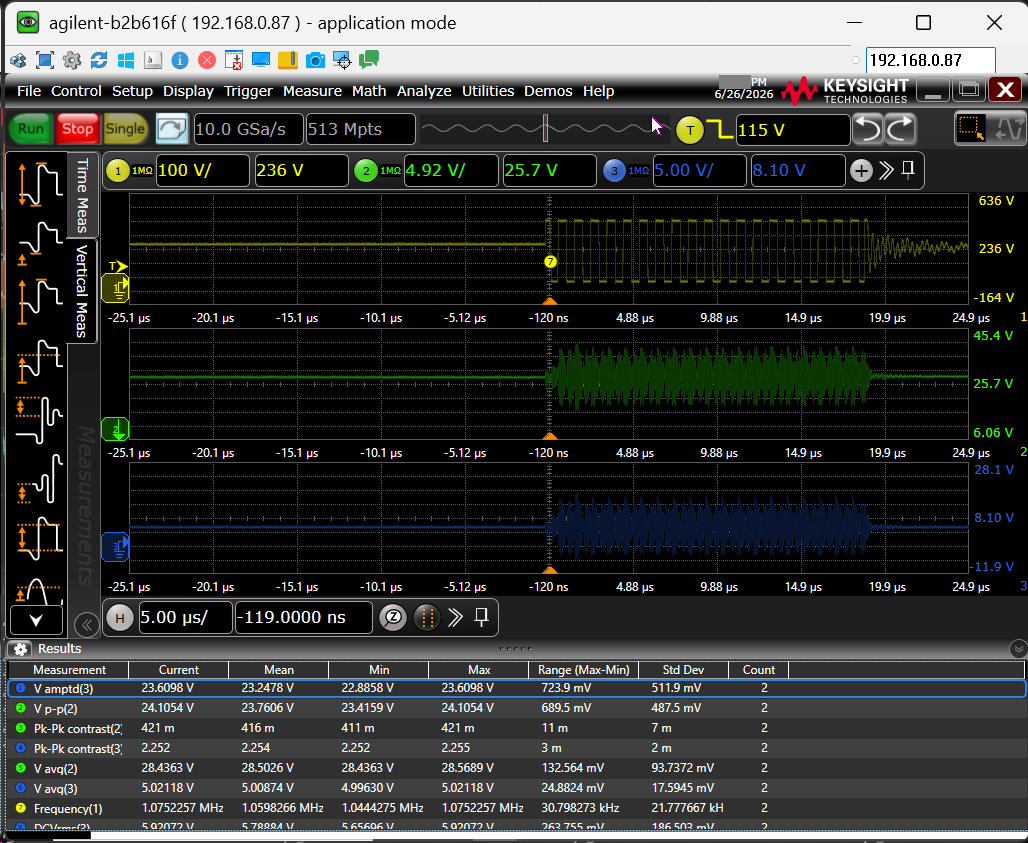
\includegraphics[width=\linewidth]{Data/measurements/evidence/PDO5_15W_3A/keysight_5v_3a_sw_secondary_vbus.png}
\caption{\SI{5}{\volt}, \SI{3}{\ampere}; \sourcefile{PDO5-MAX3A-001}.}
\end{subfigure}\hfill
\begin{subfigure}[t]{0.48\textwidth}
\centering
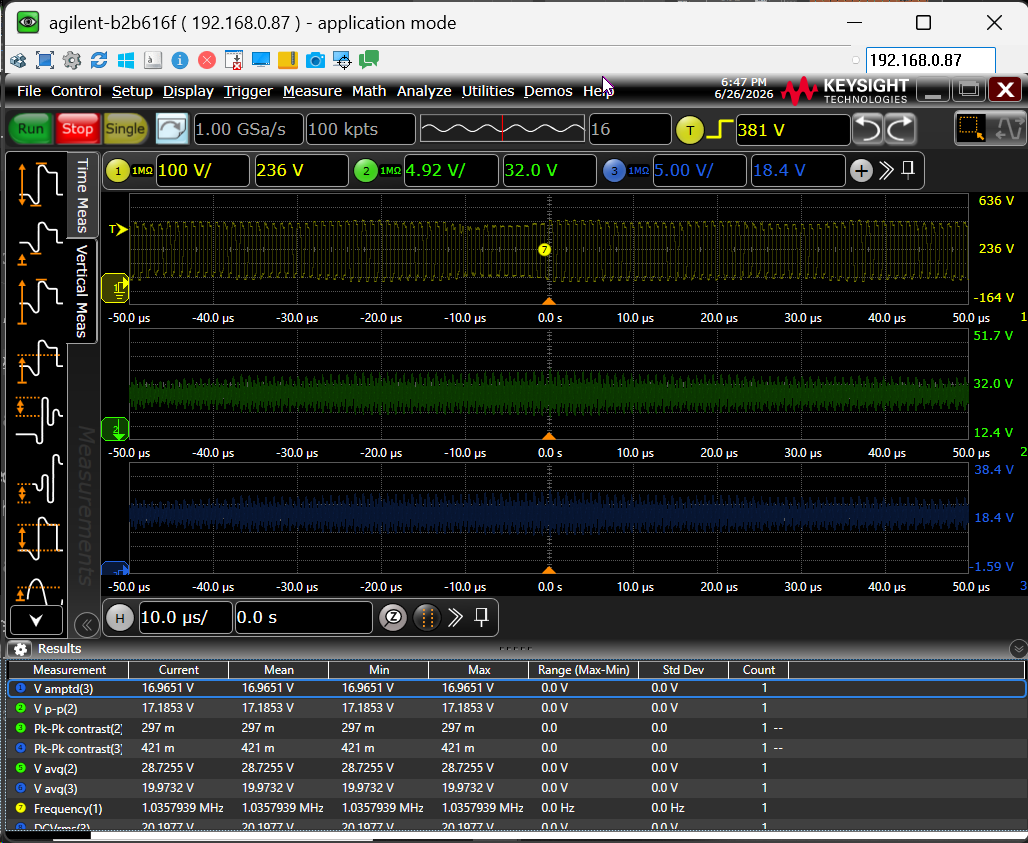
\includegraphics[width=\linewidth]{Data/measurements/evidence/PDO20_80W_40A/keysight_sw_secondary_vbus_20v_40a.png}
\caption{\SI{20}{\volt}, \SI{4}{\ampere}; \sourcefile{PDO20-80W-40A-001}.}
\end{subfigure}
\caption{DC-coupled voltage captures. Yellow: half-bridge switch-node voltage. Green: secondary output voltage. Blue: USB-C VBUS output voltage.}
\label{fig:pdo5-load-sweep-scope}
\label{fig:pdo20-high-power-scope}
\end{figure}

Long-window ripple fields remain unresolved. At \SI{20}{\volt} and
\SI{0.25}{\ampere}, VBUS is listed as \SI{12.6564}{\volt}
``amplitude/ripple.'' Several other pp entries are anomalously large.
The probe, selected measurement, and acquisition window were not fully
recorded, so these values cannot be corrected reliably and must be remeasured.

\subsection{AC-coupled detail captures}

\begin{figure}[htbp]
\centering
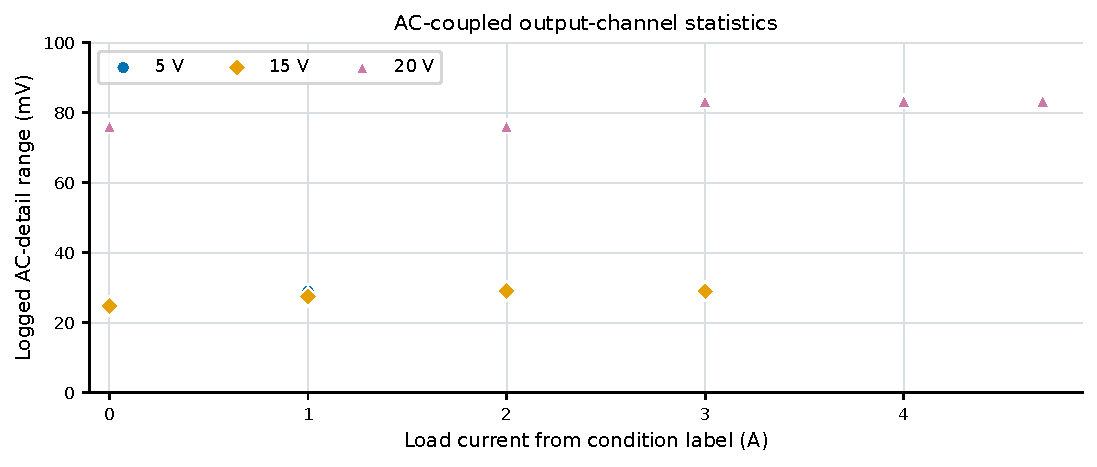
\includegraphics[width=0.95\textwidth]{Pictures/Thesis/10_Results/Rebuilt/ac_detail_statistics.pdf}
\caption{Output-channel statistics from the AC-coupled captures. Several readings are the range of average voltage across acquisitions, rather than instantaneous peak-to-peak ripple.}
\label{fig:rebuilt-ac-detail}
\end{figure}

The later AC-coupled captures used a different probe setup and report VBUS
detail fields of approximately \SI{25}{\milli\volt} to \SI{83}{\milli\volt}.
Several fields are the acquisition-to-acquisition \emph{Range (Max--Min)} of
\emph{V avg}. At \SI{5}{\volt}, \SI{3}{\ampere}, the reported
\SI{29.6924}{\milli\volt} is this statistical spread, rather than
\SI{29.7}{\milli\volt} instantaneous peak-to-peak ripple.

\begin{figure}[htbp]
\centering
\begin{subfigure}[t]{0.48\textwidth}
\centering
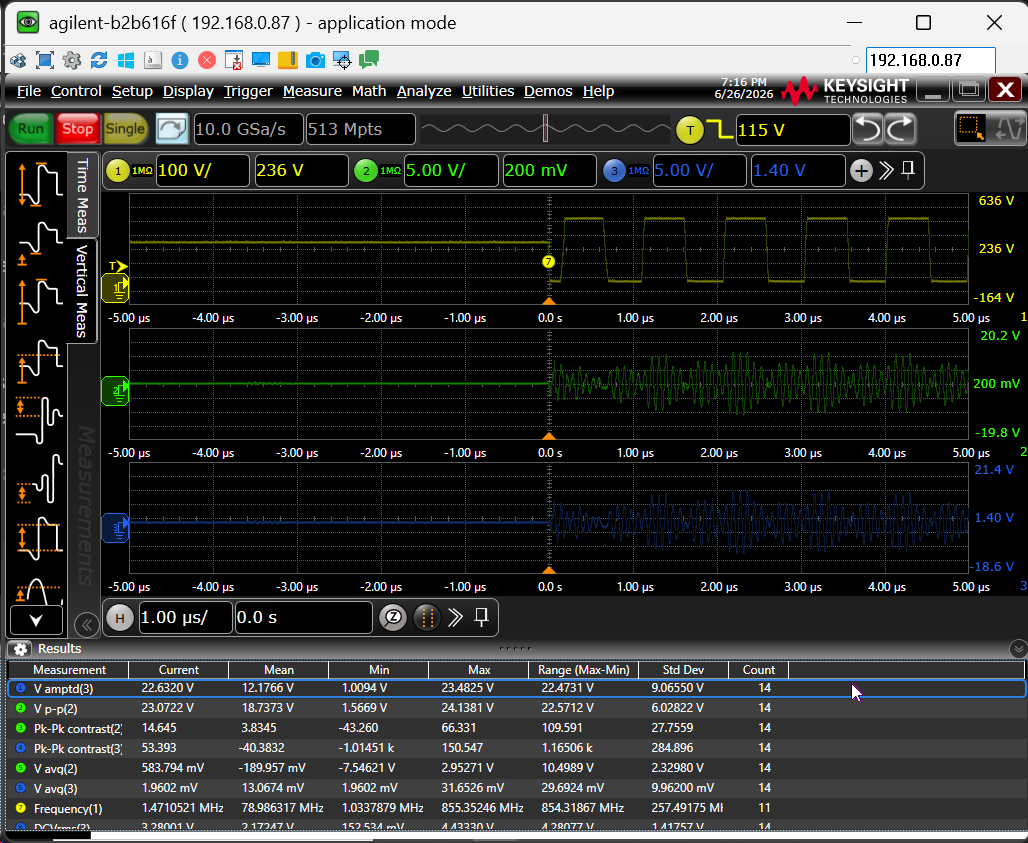
\includegraphics[width=\linewidth]{Data/measurements/evidence/PDO5_15W_3A_AC/keysight_5v_3a_ac_coupled_secondary_vbus.png}
\caption{\SI{5}{\volt}, \SI{3}{\ampere}; range of VBUS-average statistics visible.}
\end{subfigure}\hfill
\begin{subfigure}[t]{0.48\textwidth}
\centering
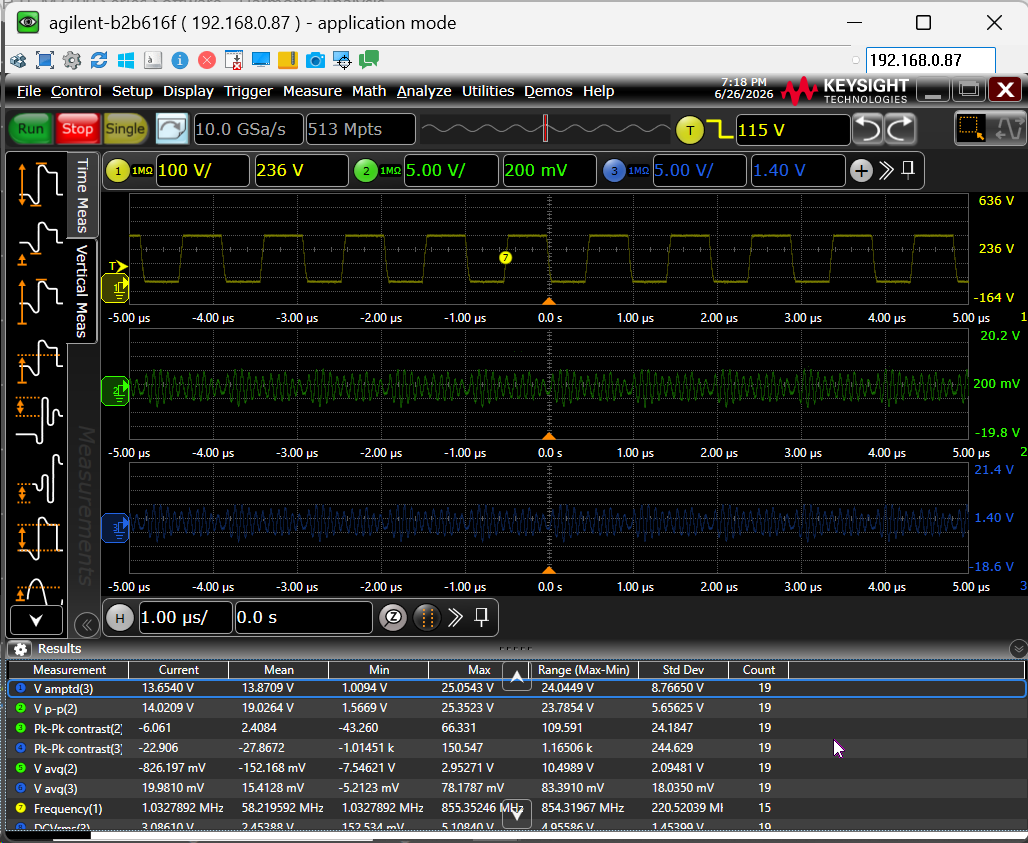
\includegraphics[width=\linewidth]{Data/measurements/evidence/PDO20_80W_4A_AC/keysight_20v_4a_ac_coupled_secondary_vbus.png}
\caption{\SI{20}{\volt}, \SI{4}{\ampere}; AC-coupled output detail.}
\end{subfigure}
\caption{Output ripple captures. Yellow: half-bridge switch-node voltage. Green: secondary output voltage. Blue: USB-C VBUS output voltage. The yellow trace is DC-coupled; the green and blue traces are AC-coupled and show voltage ripple.}
\label{fig:ac-coupled-ripple-scope}
\end{figure}

Table~\ref{tab:ac-coupled-ripple-captures-complete} includes all twelve
detail captures and their source rows. The \SI{20}{\volt},
\SI{4.7}{\ampere} entry has a nominal \SI{94}{\watt} label but no
matching DC output voltage for calculating delivered power. There is also
no completed \SI{20}{\volt}, \SI{4.5}{\ampere} test. The
\SI{20}{\volt} no-load row was excluded from the DC results because its
status is still \emph{Planned}.
